\documentclass[12pt,a4paper]{article}

% ============================================================
% PACOTES
% ============================================================
\usepackage[utf8]{inputenc}
\usepackage[T1]{fontenc}
\usepackage[brazilian]{babel}
\usepackage{amsmath,amssymb}
\usepackage{graphicx}
\usepackage{booktabs}
\usepackage{caption}
\usepackage{float}
\usepackage{geometry}
\usepackage{hyperref}
\usepackage{xcolor}
\usepackage{enumitem}
\usepackage{array}
\usepackage{longtable}

\geometry{margin=2.5cm}
\hypersetup{
    colorlinks=true,
    linkcolor=blue,
    citecolor=blue,
    urlcolor=blue
}

% ------------------------------------------------------------
% Ambiente para indicar onde cada figura/imagem deve entrar,
% sem inserir a imagem de fato. Basta trocar o conteúdo do
% \fbox por \includegraphics{caminho/da/imagem.png} depois.
% (Nomes de arquivo usam hífen, nunca underscore, para não
% quebrar a compilação em modo texto normal do LaTeX.)
% ------------------------------------------------------------
\newcommand{\figuraPendente}[3]{%
\begin{figure}[H]
    \centering
    \fbox{\begin{minipage}{0.85\textwidth}
        \centering
        \vspace{2.5cm}
        \textbf{[INSERIR FIGURA AQUI]}\\[0.3cm]
        \textit{Arquivo sugerido:} \texttt{#1}\\[0.3cm]
        \textit{Conteúdo:} #2
        \vspace{2.5cm}
    \end{minipage}}
    \caption{#3}
    \label{fig:#1}
\end{figure}
}

% ============================================================
% CABEÇALHO / TÍTULO
% ============================================================
\title{
    \Large \textbf{Avanços em Inteligência Artificial} \\
    \large EELT7025 --- PPGEE, UFPR \\[0.3cm]
    \normalsize Exercícios da Aula 02 \\
    \normalsize Estatística Descritiva e Análise de Séries Temporais
}
\author{Adriely Teixeira de Paula, Betina Zynger Capaverde, Emilio Gaudeda Junior}
\date{\today}

% ============================================================
\begin{document}

\maketitle
\tableofcontents
\newpage

% ============================================================
\section*{Datasets utilizados}
\addcontentsline{toc}{section}{Datasets utilizados}

\begin{itemize}
    \item \textbf{Exercício 1 (análise de séries temporais):} \emph{PJM Hourly Energy Consumption}, carga horária (MW) da região \textbf{PJME} (variável-alvo) e da região vizinha \textbf{PJMW} (variável exógena numérica), 2002--2018.
    \item \textbf{Exercício 2 (classificação de séries temporais):} \emph{ItalyPowerDemand}, curvas diárias (24 pontos horários) de demanda elétrica italiana, rotuladas como período Out--Mar (classe 1) ou Abr--Set (classe 2), do UCR/UEA Time Series Classification Archive.
\end{itemize}

\newpage
% ============================================================
% EXERCÍCIO 1
% ============================================================
\section{Exercício 1 --- Análise de Séries Temporais (PJM Hourly Energy Consumption)}

\subsection{Carregamento e período coberto}

\begin{table}[H]
\centering
\caption{Resumo do carregamento dos dados}
\begin{tabular}{lccc}
\toprule
Série & Nº de registros & Início & Fim \\
\midrule
PJME (alvo)     & 145.366 & 2002-01-01 01:00 & 2018-08-03 00:00 \\
PJMW (exógena)  & 143.206 & 2002-04-01 01:00 & 2018-08-03 00:00 \\
\bottomrule
\end{tabular}
\end{table}

\subsection{Checklist de qualidade dos dados}

\begin{itemize}
    \item \textbf{Duplicatas de timestamp:} 4 duplicatas efetivas, sempre em início de novembro às 02:00, artefato do horário de verão (DST \emph{fall-back}) nos EUA.
    \item \textbf{Lacunas de timestamp:} 30 timestamps ausentes no índice horário completo, concentrados em março/abril às 02:00--03:00, horas que ``somem'' no DST \emph{spring-forward}.
    \item \textbf{Mecanismo dos dados ausentes:} MCAR (\emph{Missing Completely At Random}), a ausência segue uma regra de calendário externa e determinística, não depende do valor da própria demanda.
    \item \textbf{Plausibilidade de escala:} PJME entre 14.544 e 62.009 MW (média 32.080 MW); PJMW entre 487 e 9.594 MW (média 5.602 MW). Nenhum valor negativo ou nulo suspeito.
    \item \textbf{Tratamento aplicado:} reindexação para frequência horária completa + interpolação linear das lacunas. Série final: 145.392 observações, 0 ausentes, 0 duplicatas.
\end{itemize}

\subsection{Análise univariada da carga (PJME)}

\begin{table}[H]
\centering
\caption{Estatísticas descritivas --- Carga PJME (MW)}
\begin{tabular}{lc}
\toprule
Estatística & Valor \\
\midrule
Média              & 32.078,9 MW \\
Mediana            & 31.420,0 MW \\
Desvio-padrão      & 6.464,3 MW \\
Q1 / Q3            & 27.571,0 / 35.647,0 MW \\
IQR                & 8.076,0 MW \\
Mínimo / Máximo    & 14.544,0 / 62.009,0 MW \\
Assimetria (\emph{skew}) & 0{,}739 (à direita) \\
Curtose (excesso)  & 0{,}736 (leptocúrtica) \\
\bottomrule
\end{tabular}
\end{table}


\begin{figure}[H]
    \centering
    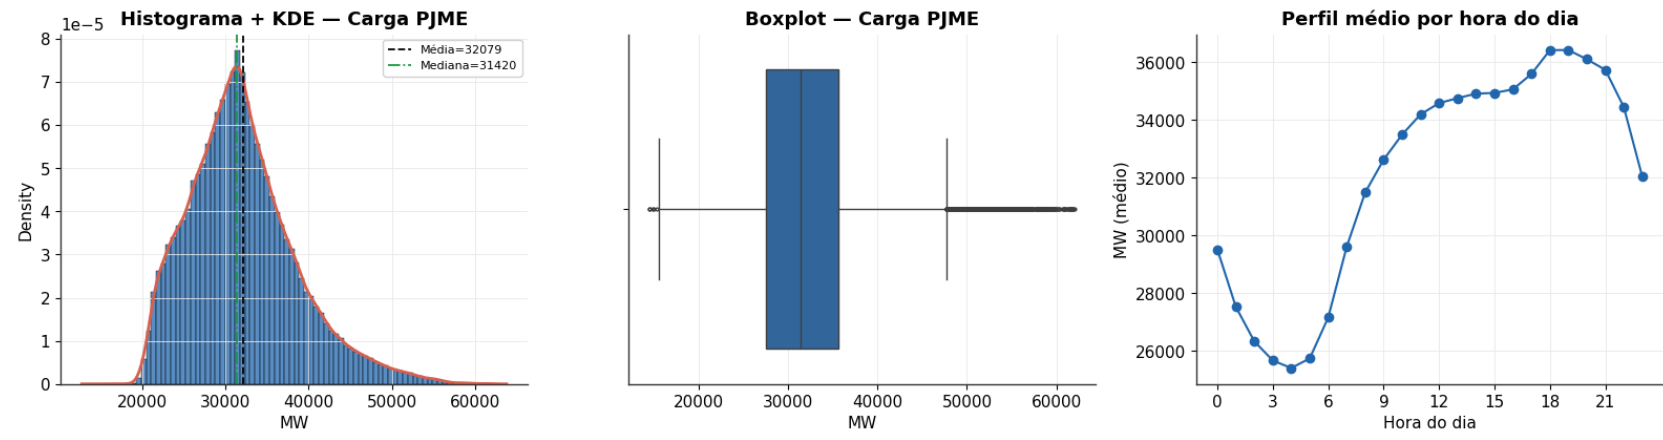
\includegraphics[width=0.85\textwidth]{Figuras_Aula2/fig1-histograma-boxplot-perfil.png}
    \caption{Análise univariada da carga PJME --- histograma, boxplot e perfil horário.}
    \label{fig:fig1}
\end{figure}

\subsection{Detecção de outliers --- IQR vs. Z-score Modificado (MAD)}

\begin{table}[H]
\centering
\caption{Comparação de métodos de detecção de outliers}
\begin{tabular}{lcc}
\toprule
Método & Nº de outliers & \% dos dados \\
\midrule
IQR (limites [15.457, 47.761] MW) & 3.460 & 2{,}380\% \\
Z-score Modificado (MAD, $|Z_{mod}|>3{,}5$) & 1.003 & 0{,}690\% \\
\midrule
Sinalizados por ambos os métodos & \multicolumn{2}{c}{1.003} \\
Sinalizados só pelo IQR & \multicolumn{2}{c}{2.457} \\
Sinalizados só pelo MAD & \multicolumn{2}{c}{0} \\
\bottomrule
\end{tabular}
\end{table}


\begin{figure}[H]
    \centering
    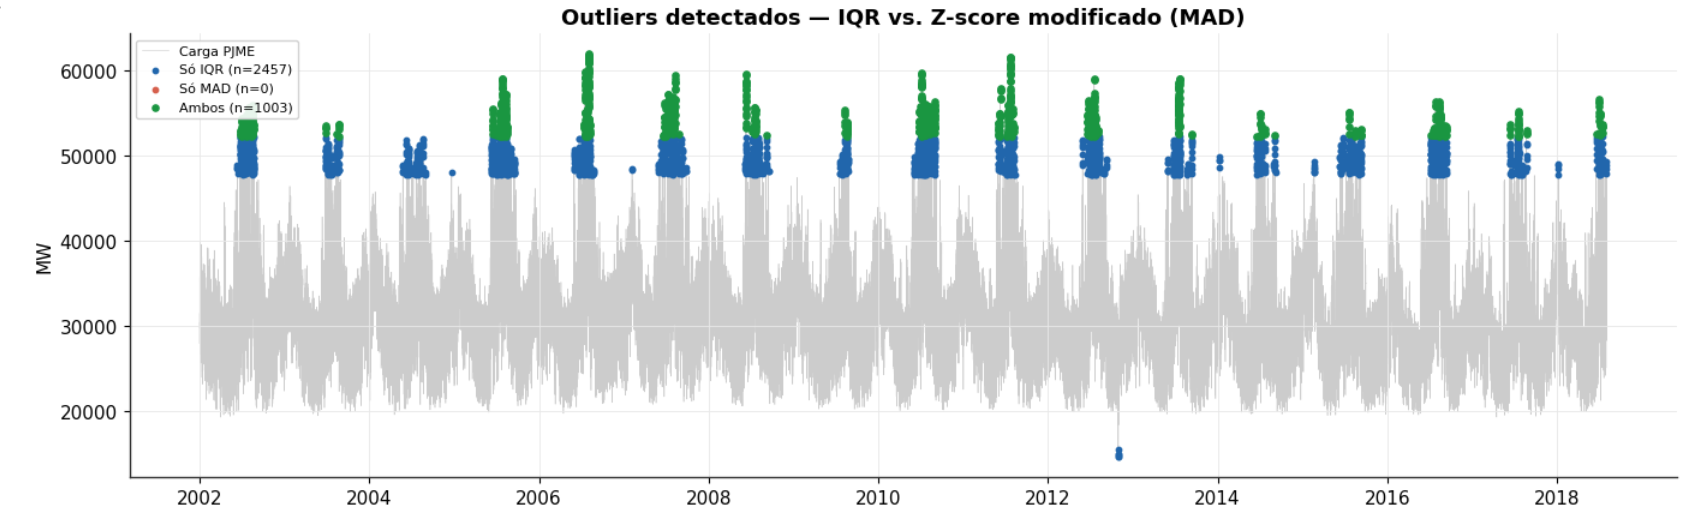
\includegraphics[width=0.85\textwidth]{Figuras_Aula2/fig2-outliers-iqr-mad.png}
    \caption{Outliers detectados --- IQR vs. Z-score Modificado (MAD).}
    \label{fig:fig1}
\end{figure}

\subsection{Correlação com variável exógena (PJMW) e tamanho de efeito}

\begin{table}[H]
\centering
\caption{Correlação PJME (alvo) vs. PJMW (exógena) --- período comum $n=143.232$}
\begin{tabular}{lcc}
\toprule
Coeficiente & Valor & p-valor \\
\midrule
Pearson $r$   & 0{,}8757 & $<10^{-300}$ \\
Spearman $\rho$ & 0{,}8890 & $<10^{-300}$ \\
Kendall $\tau$  & 0{,}7085 & $<10^{-300}$ (amostra de 20.000 pontos) \\
\bottomrule
\end{tabular}
\end{table}

\begin{figure}[H]
    \centering
    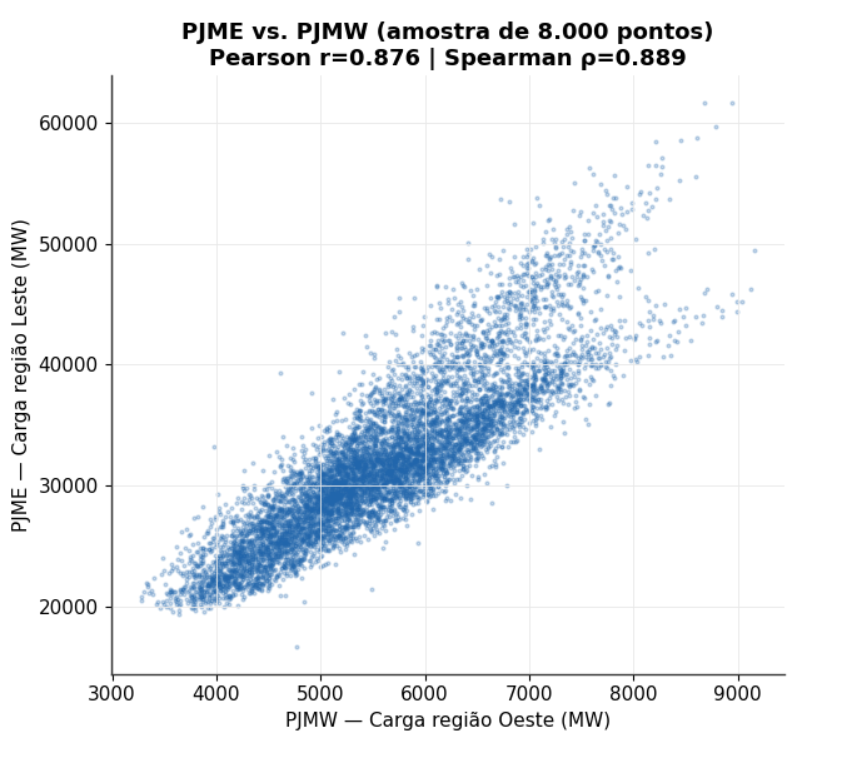
\includegraphics[width=0.85\textwidth]{Figuras_Aula2/fig3-scatter-pjme-pjmw.png}
    \caption{Dispersão PJME vs. PJMW --- correlação entre regiões.}
    \label{fig:fig1}
\end{figure}


\begin{table}[H]
\centering
\caption{Tamanho de efeito --- horário de pico (17h--20h) vs. fora de pico (2h--5h)}
\begin{tabular}{lc}
\toprule
Grandeza & Valor \\
\midrule
Média horário de pico ($n=24.232$)    & 36.137,9 MW \\
Média fora de pico ($n=24.232$)       & 25.795,4 MW \\
Teste $t$ de Welch                    & $t=216{,}9$, $p<10^{-300}$ \\
Cohen's $d$                           & 1{,}970 (efeito grande) \\
\bottomrule
\end{tabular}
\end{table}

\subsection{Média móvel, desvio-padrão móvel e 1ª diferença}

\begin{itemize}
    \item Desvio-padrão da 1ª diferença: 1.451,9 MW vs. 6.464,3 MW da série bruta, a diferenciação remove grande parte da variação de baixa frequência.
    \item A média móvel (janela 24h) suaviza o ciclo diário e revela tendência/sazonalidade de mais baixa frequência (semanal, sazonal).
    \item O desvio-padrão móvel tende a subir em transições de estação e em ondas de calor/frio.
\end{itemize}

\begin{figure}[H]
    \centering
    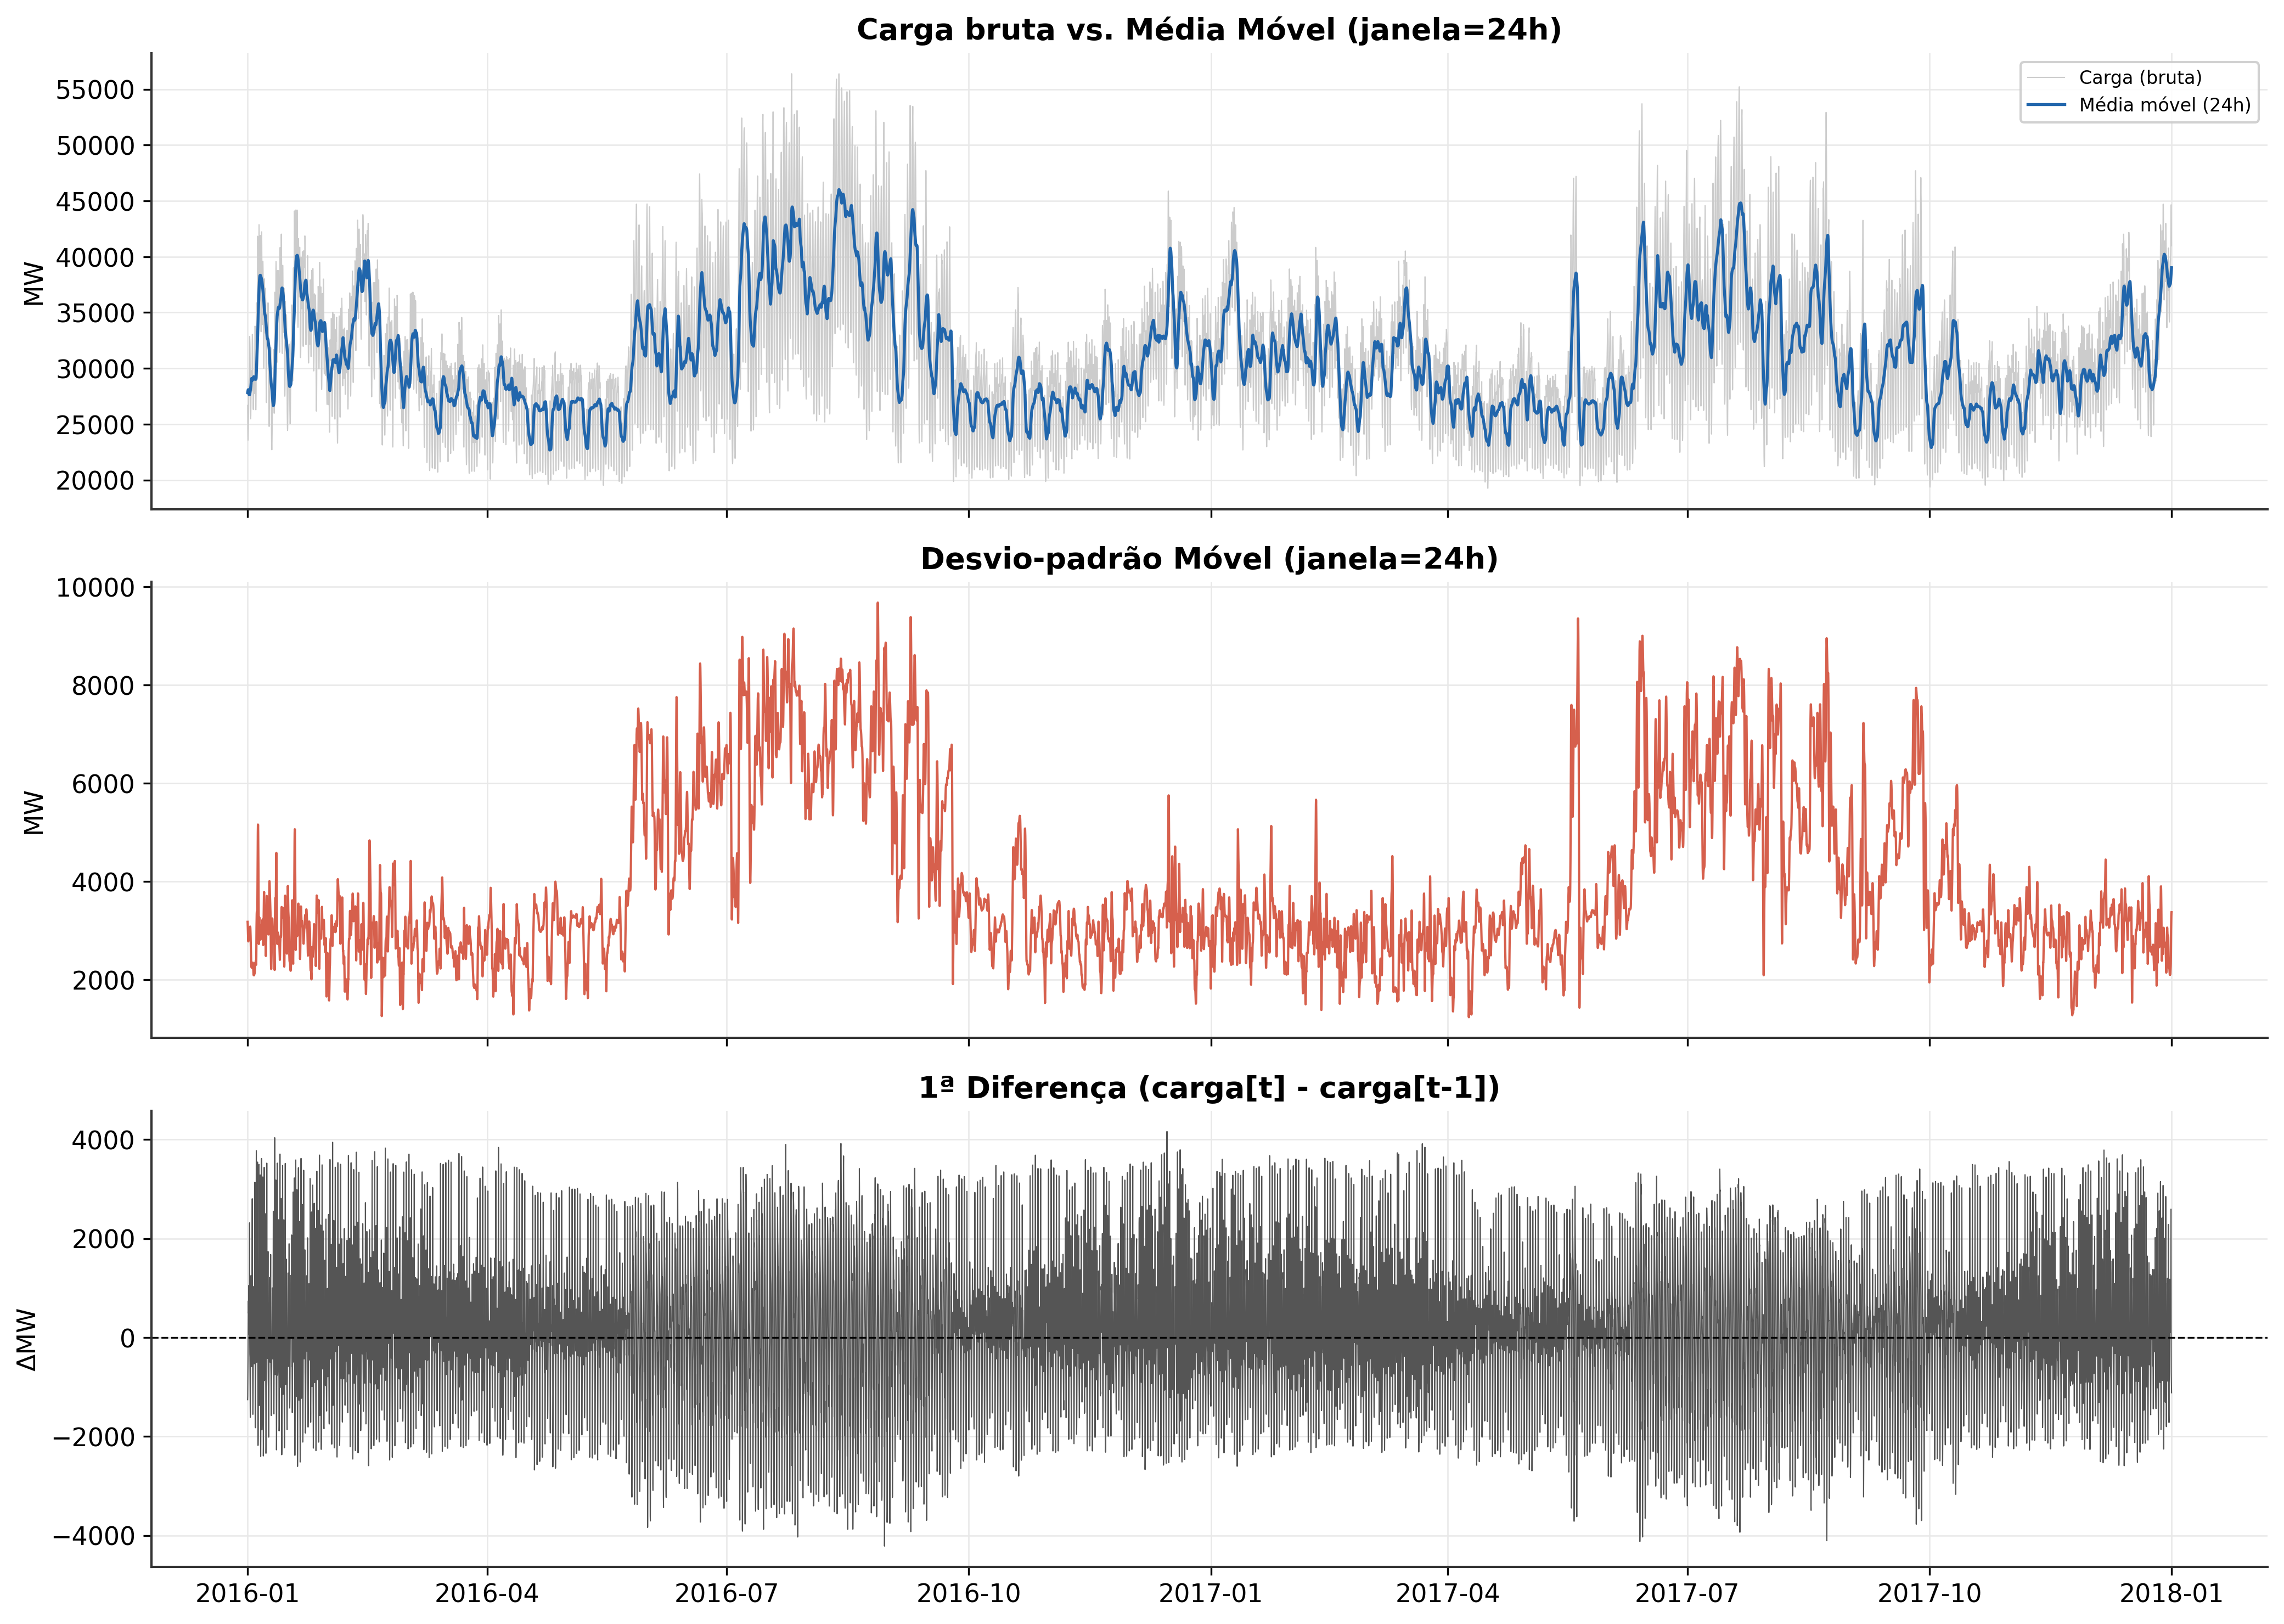
\includegraphics[width=0.85\textwidth]{Figuras_Aula2/fig4-media-movel-diff.png}
    \caption{Média móvel, desvio-padrão móvel e 1ª diferença --- Carga PJME.}
    \label{fig:fig1}
\end{figure}


\subsection{Decomposição STL e forças de tendência/sazonalidade}

\begin{table}[H]
\centering
\caption{STL --- variância explicada por componente (sazonalidade diária, \texttt{period=24})}
\begin{tabular}{lcc}
\toprule
Componente & Variância & \% da var. total \\
\midrule
Tendência    & 19.418.383 & 46{,}5\% \\
Sazonalidade & 18.965.600 & 45{,}4\% \\
Resíduo      &  2.756.443 &  6{,}6\% \\
\bottomrule
\end{tabular}
\end{table}

\noindent Força de Tendência $F_T = 0{,}8850$ \quad|\quad Força de Sazonalidade $F_S = 0{,}8660$.

\begin{figure}[H]
    \centering
    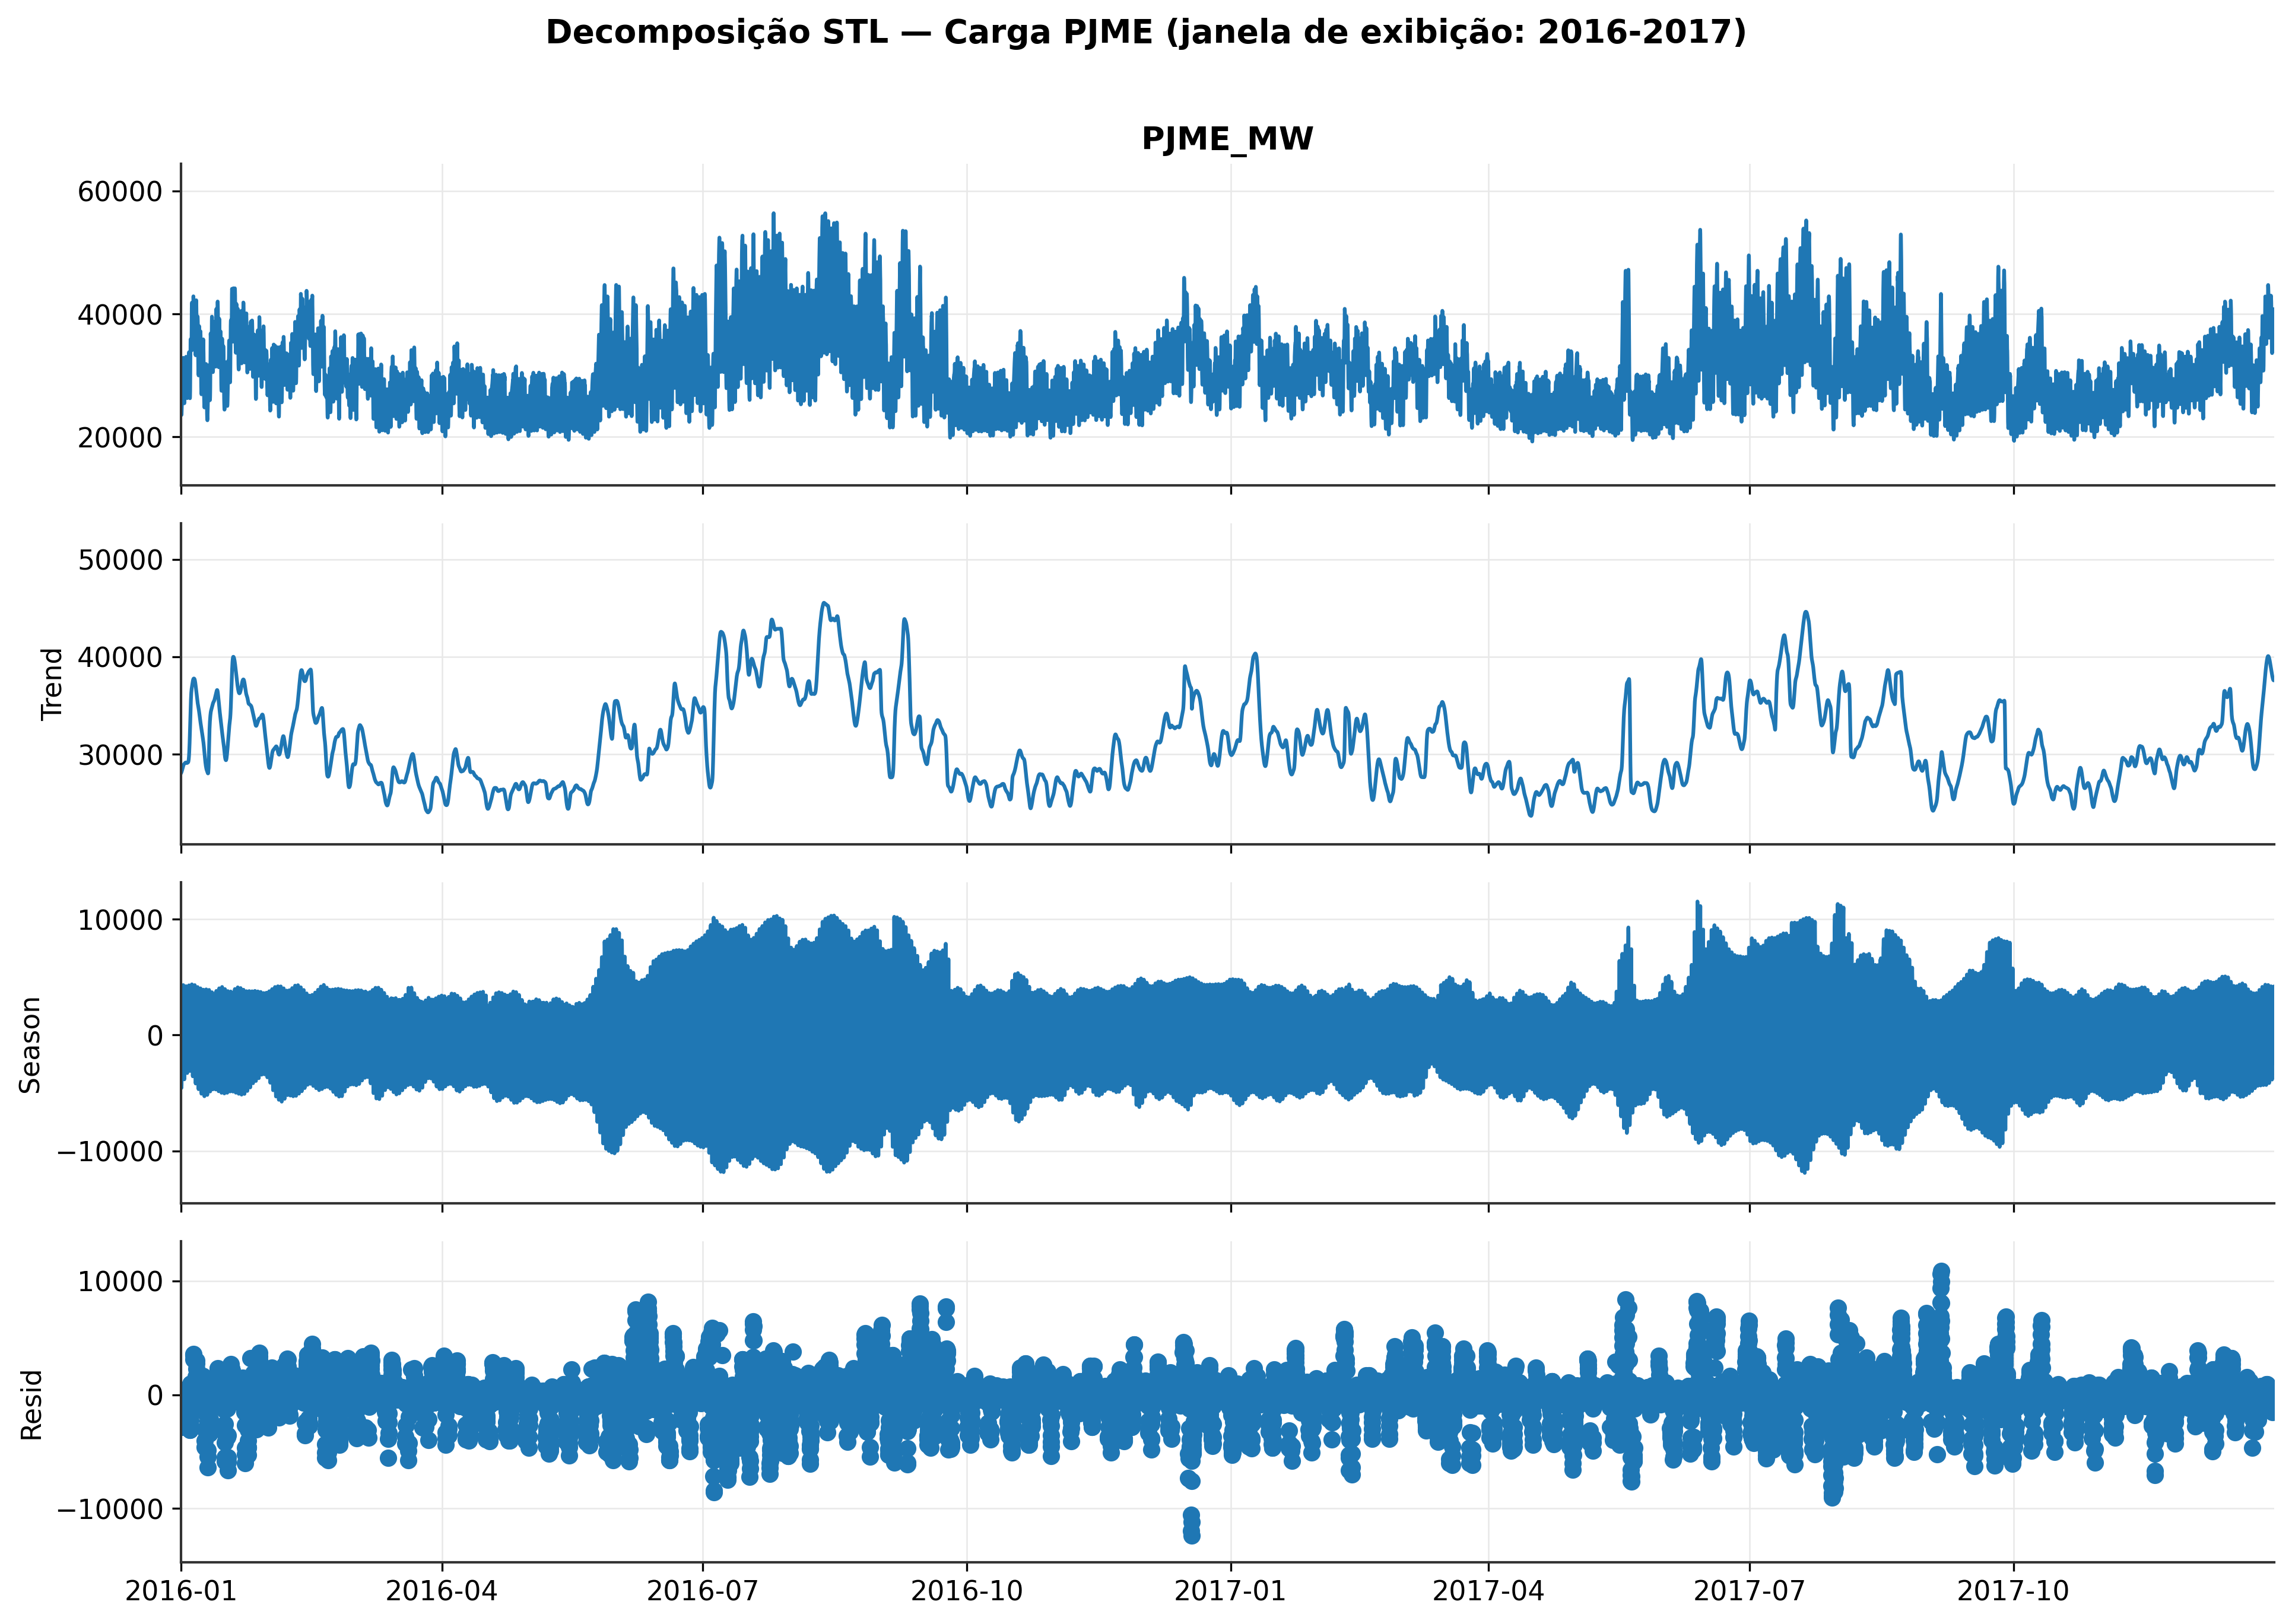
\includegraphics[width=0.85\textwidth]{Figuras_Aula2/fig5-decomposicao-stl.png}
    \caption{Decomposição STL --- Carga PJME.}
    \label{fig:fig1}
\end{figure}


\newpage
% ============================================================
% EXERCÍCIO 2 (continuação do PJM: itens 6-13 do roteiro original)
% ============================================================
\section{Continuação --- Padrões Cíclicos, Autocorrelação, Frequência e Estacionariedade (PJM)}

\subsection{Autocorrelação (ACF) e Autocorrelação Parcial (PACF)}

\begin{figure}[H]
    \centering
    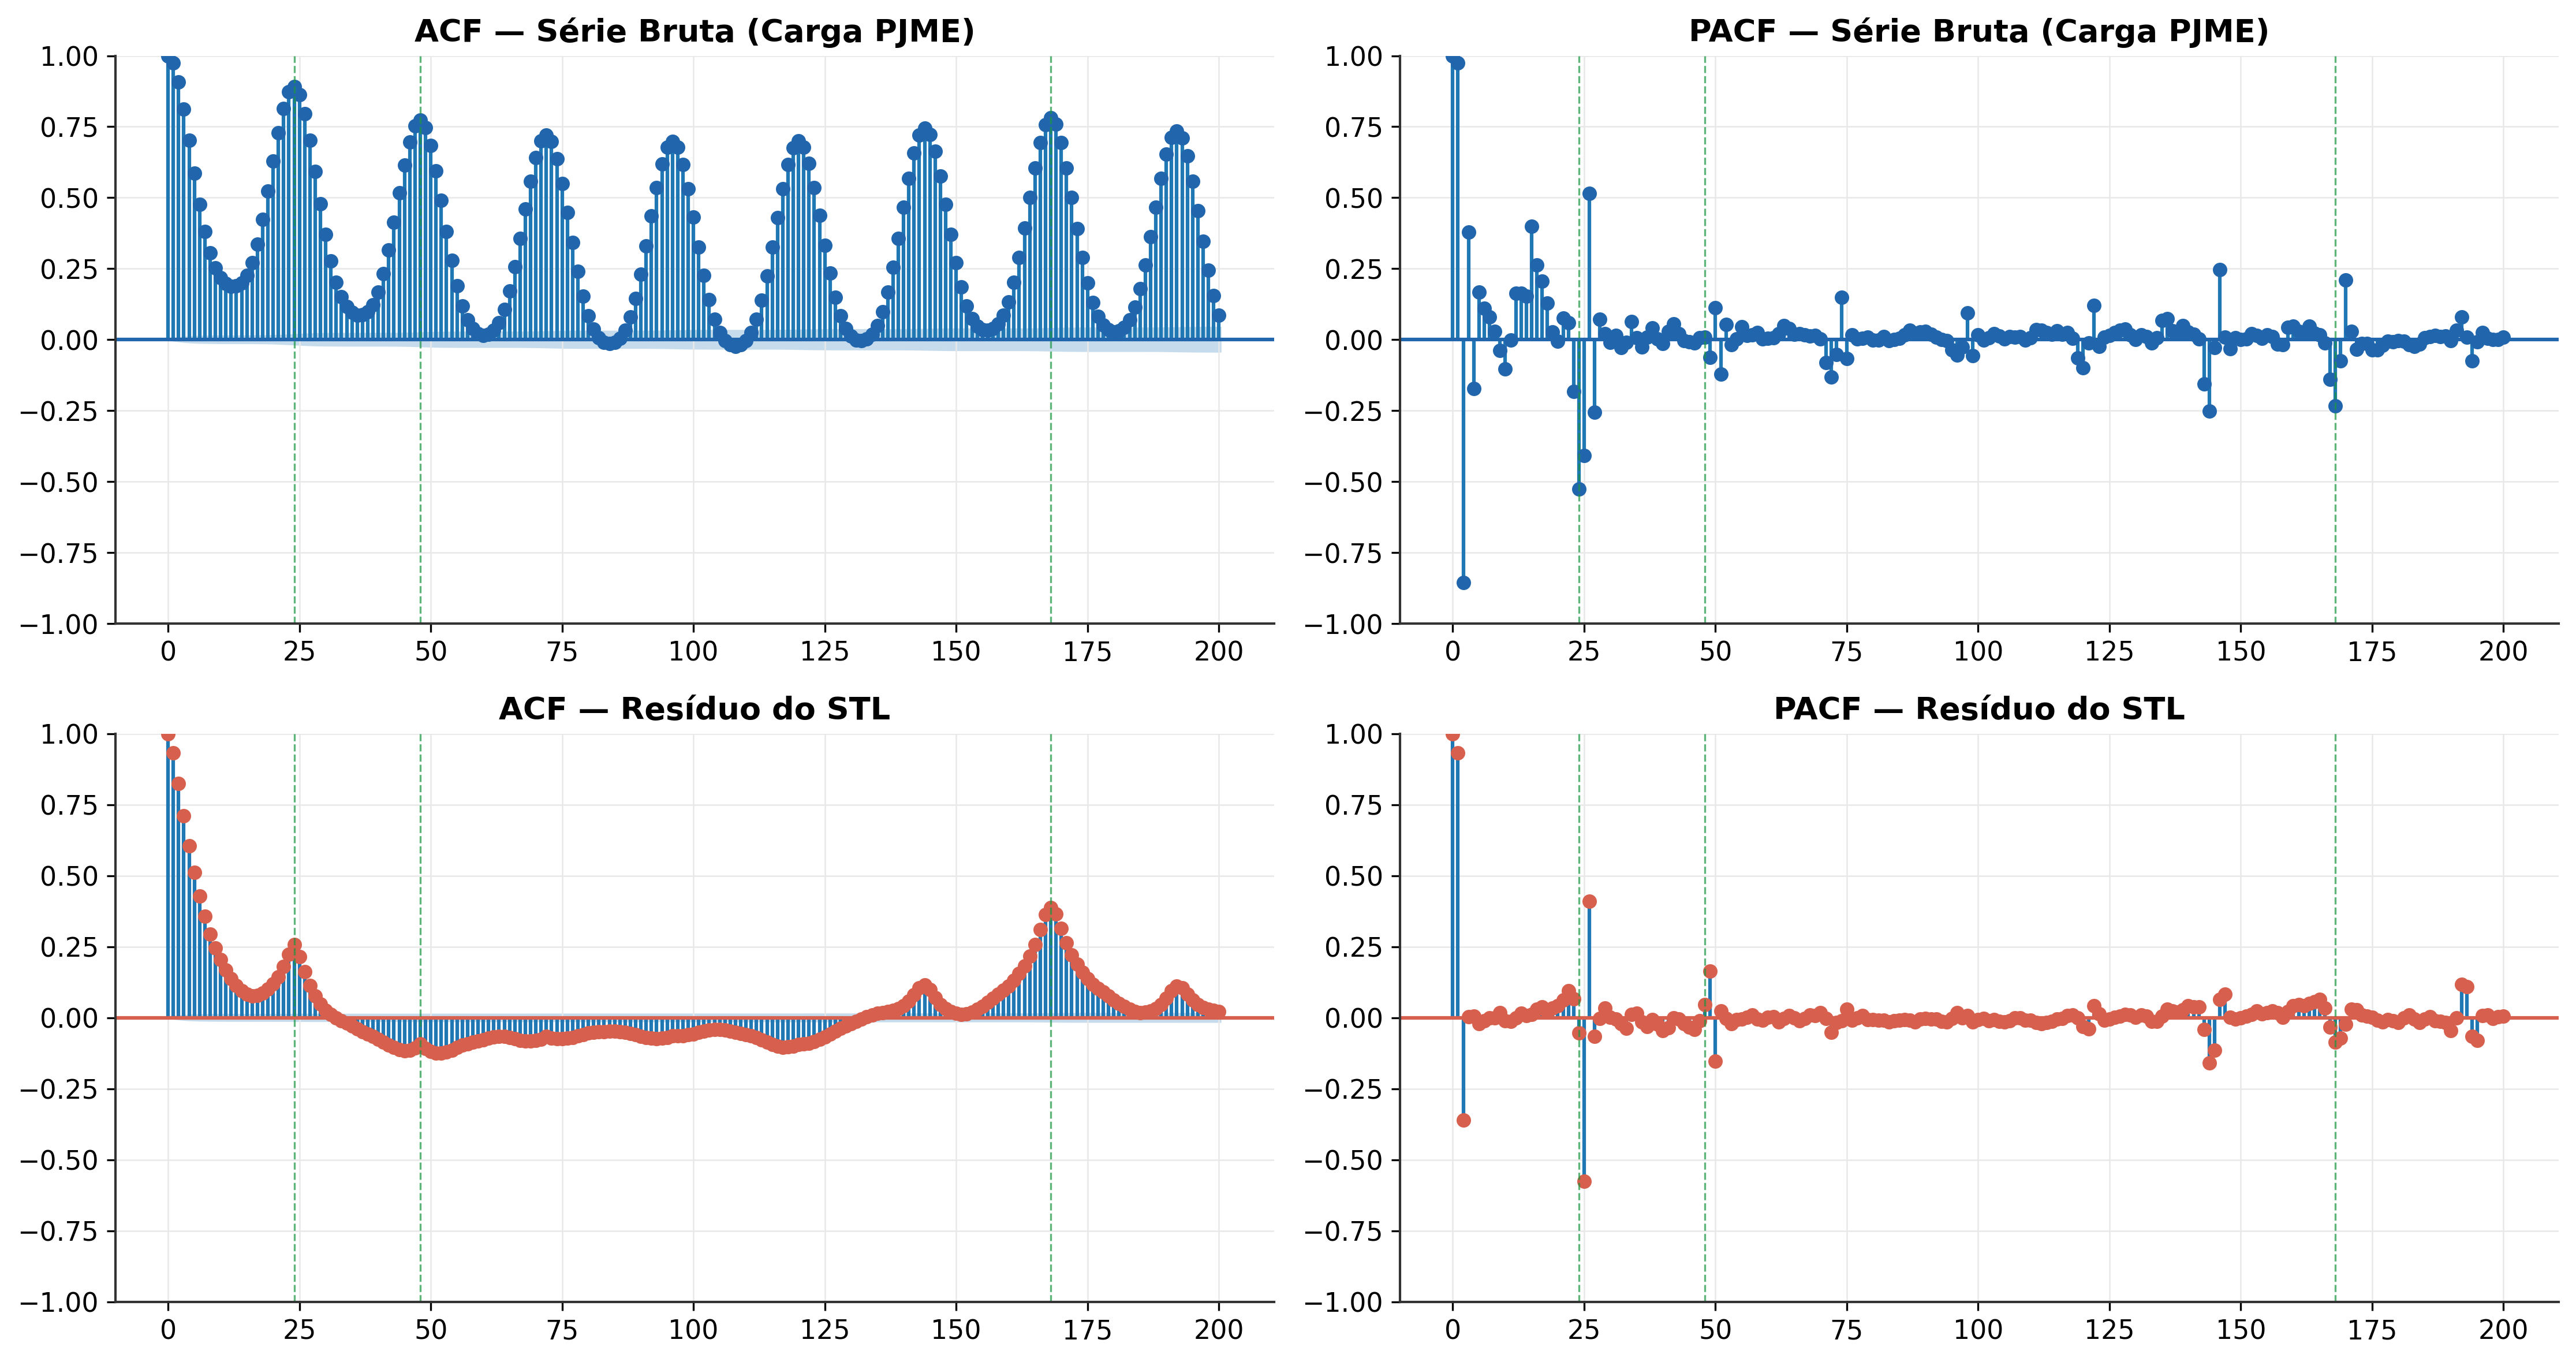
\includegraphics[width=0.85\textwidth]{Figuras_Aula2/fig6-acf-pacf.png}
    \caption{ACF/PACF --- série bruta e resíduo do STL.}
    \label{fig:fig1}
\end{figure}

\noindent A ACF mostra picos fortes e persistentes em múltiplos de 24h e em 168h (1 semana), dupla sazonalidade diária+semanal. Mesmo após a decomposição STL (\texttt{period=24}), o resíduo ainda apresenta autocorrelação relevante no lag 168, indicando que a sazonalidade semanal não foi capturada.

\subsection{Teste de Ljung-Box}

\begin{table}[H]
\centering
\caption{Ljung-Box --- série bruta vs. resíduo do STL}
\begin{tabular}{lcccc}
\toprule
& \multicolumn{2}{c}{Série bruta} & \multicolumn{2}{c}{Resíduo do STL} \\
Lag & Estatística & p-valor & Estatística & p-valor \\
\midrule
24  & 1.139.160 & 0{,}0 & 505.527 & 0{,}0 \\
48  & 1.930.233 & 0{,}0 & 534.425 & 0{,}0 \\
168 & 4.744.568 & 0{,}0 & 696.955 & 0{,}0 \\
\bottomrule
\end{tabular}
\end{table}

\noindent Em ambos os casos, $p\approx 0$ em todos os lags: mesmo após a remoção da sazonalidade diária, o resíduo ainda contém autocorrelação estatisticamente significativa (sazonalidade semanal residual).

\subsection{Espectro de potência (FFT/Periodograma)}


\begin{figure}[H]
    \centering
    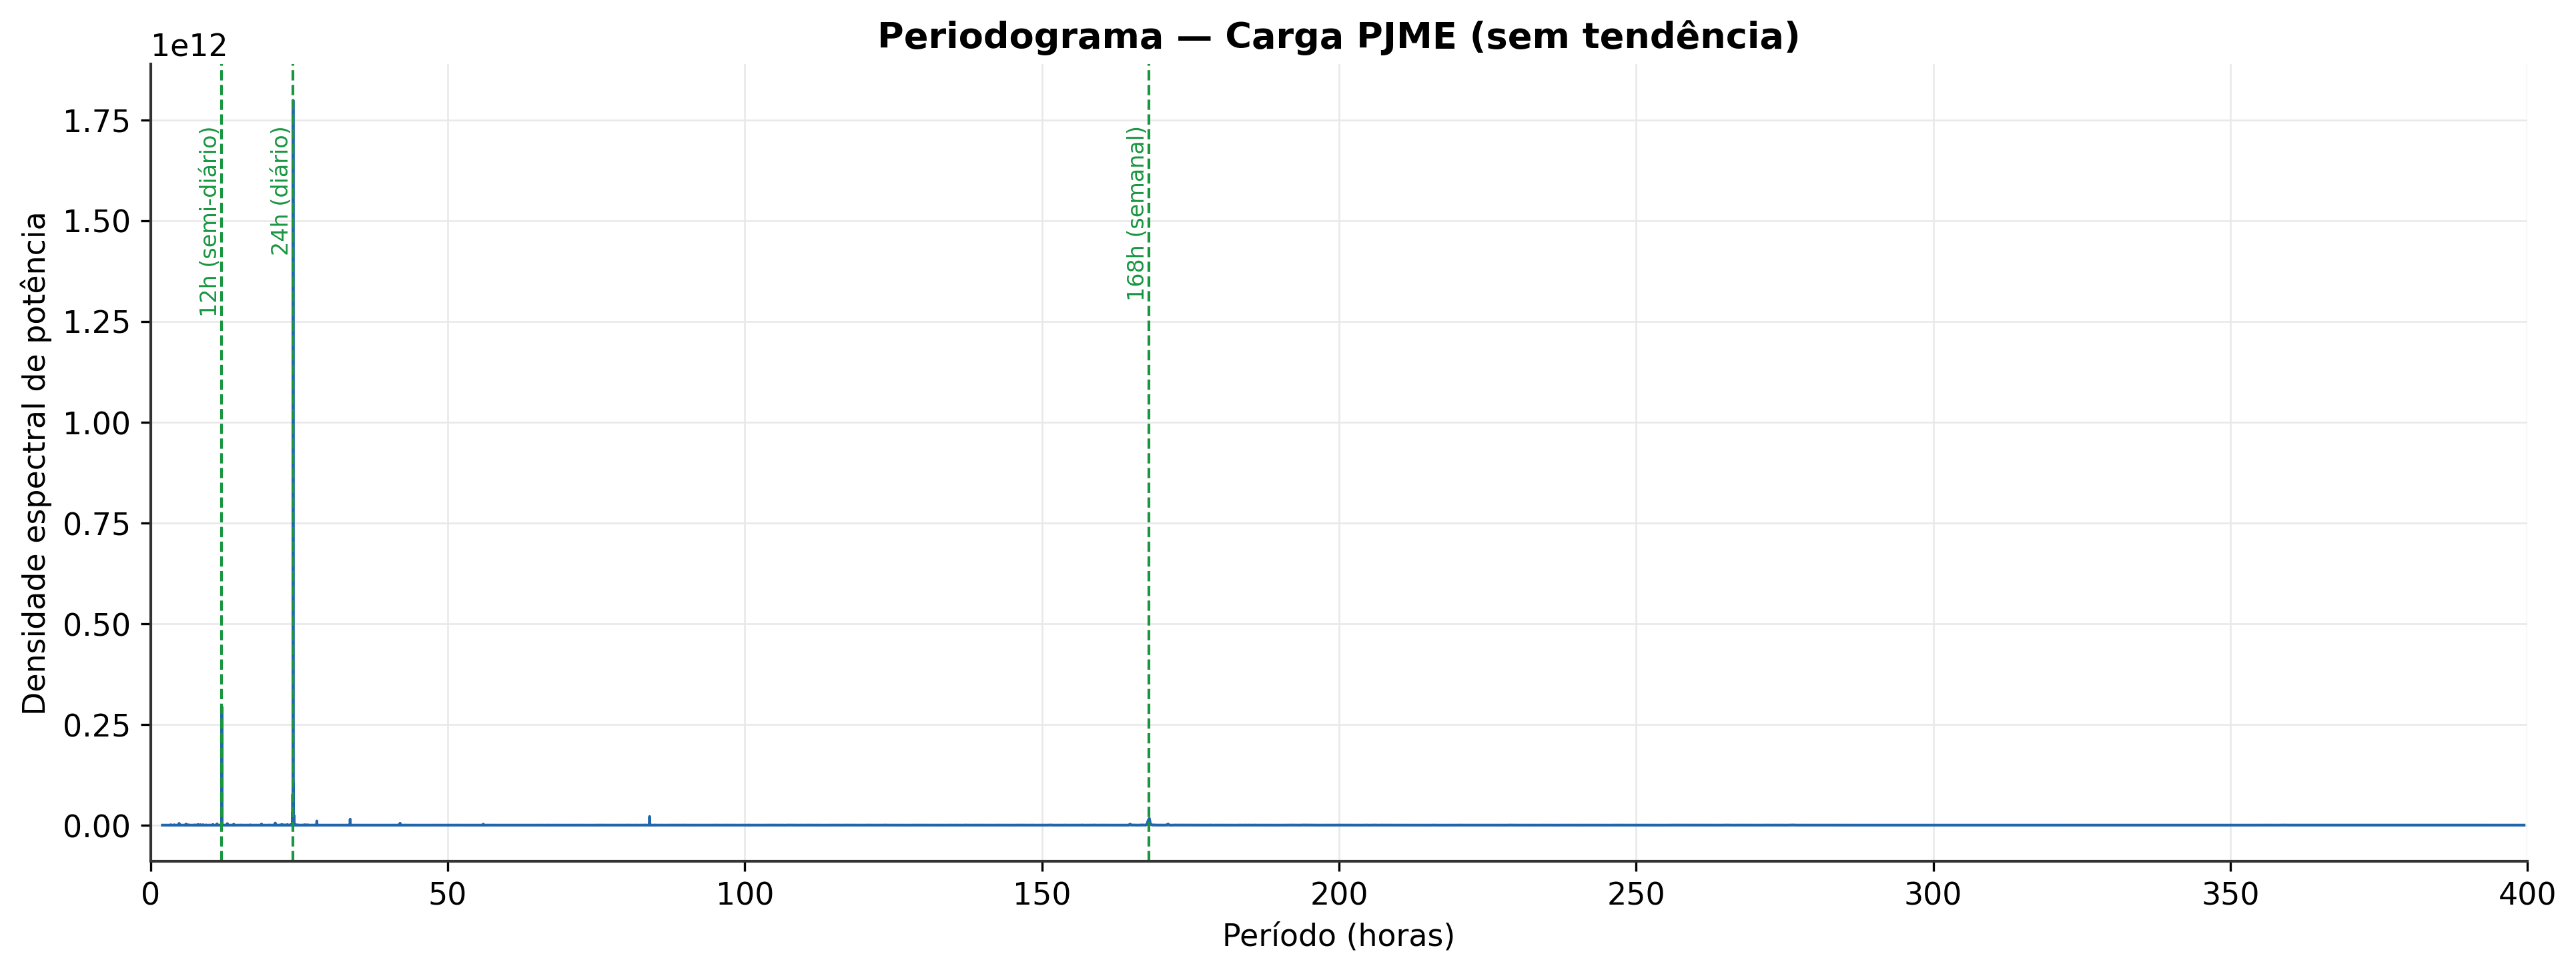
\includegraphics[width=0.85\textwidth]{Figuras_Aula2/fig7-periodograma.png}
    \caption{Periodograma --- Carga PJME (sem tendência).}
    \label{fig:fig1}
\end{figure}

\noindent O periodograma confirma os mesmos picos da ACF/PACF: período dominante de 24h (ciclo diário), harmônico em 12h, e pico nítido em 168h (ciclo semanal), concordância entre os domínios do tempo e da frequência.

\subsection{Estacionariedade --- ADF e KPSS}

\begin{table}[H]
\centering
\caption{Diagnóstico combinado ADF + KPSS}
\begin{tabular}{lcccccc}
\toprule
Série & ADF stat & ADF $p$ & ADF estac.? & KPSS stat & KPSS $p$ & Veredito \\
\midrule
Bruta          & $-24{,}88$ & 0{,}0 & Sim & 3{,}54 & 0{,}01 & Conflito ADF$\times$KPSS \\
1ª diferença   & $-66{,}12$ & 0{,}0 & Sim & 0{,}0007 & 0{,}10 & Estacionária (concordam) \\
Resíduo STL    & $-48{,}33$ & 0{,}0 & Sim & 2{,}09 & 0{,}01 & Conflito ADF$\times$KPSS \\
\bottomrule
\end{tabular}
\end{table}

\noindent O conflito ADF$\times$KPSS na série bruta e no resíduo do STL é o padrão esperado para séries com sazonalidade determinística forte (sazonalidade semanal remanescente); a 1ª diferença satisfaz ambos os testes simultaneamente.

\subsection{Tabela-síntese --- EDA $\rightarrow$ decisões de modelagem}

\begin{table}[H]
\centering
\small
\begin{tabular}{p{6.5cm}p{7.5cm}}
\toprule
\textbf{Achado da EDA} & \textbf{Decisão de modelagem} \\
\midrule
Duplicatas/lacunas ligadas ao DST & Consolidar duplicatas e interpolar lacunas antes de qualquer modelagem \\
Assimetria à direita, caudas pesadas & Considerar erro robusto (MAE/Huber) em vez de resíduos gaussianos \\
Poucos outliers extremos concordantes (IQR/MAD) & Sinalizar como \emph{feature} em vez de remover \\
Correlação forte com PJMW & Incluir carga da região vizinha como covariável exógena \\
Cohen's $d$ muito grande (pico vs. fora de pico) & Incluir hora do dia como \emph{feature} categórica forte \\
$F_S\approx 1$; $F_T$ moderada & Modelar sazonalidade diária explicitamente (Fourier/dummies horárias) \\
ACF/PACF/FFT: picos em 24h/12h/168h & Usar lags 24, 48, 168; considerar dupla sazonalidade (MSTL) \\
Ljung-Box rejeita mesmo no resíduo do STL & Adotar STL com múltiplas sazonalidades ou sazonalidade semanal explícita \\
ADF$\times$KPSS discordam na série bruta & Diferenciar a série antes de modelos que assumem estacionariedade \\
\bottomrule
\end{tabular}
\caption{Síntese, da EDA às decisões de modelagem (PJM Hourly Energy Consumption)}
\end{table}

\newpage
% ============================================================
% EXERCÍCIO 2 (ItalyPowerDemand)
% ============================================================
\section{Exercício 2 --- Classificação de Séries Temporais (ItalyPowerDemand)}

\subsection{Descrição do problema}

\begin{itemize}
    \item \textbf{Unidade de análise:} cada instância é uma série temporal completa --- curva diária de demanda elétrica italiana com 24 pontos horários.
    \item \textbf{Classes:} 2 --- dias de Outubro a Março (classe 1, semestre frio) vs. Abril a Setembro (classe 2, semestre quente).
    \item \textbf{Interpretação física:} classificar o \emph{formato} da curva de carga diária (série padronizada por instância) como típico de inverno ou de verão.
\end{itemize}

\subsection{Balanceamento das classes}

\begin{table}[H]
\centering
\caption{Balanceamento das classes --- ItalyPowerDemand}
\begin{tabular}{lcc}
\toprule
Classe & Nº de séries & \% do total \\
\midrule
1 (Out--Mar) & 547 & 49{,}9\% \\
2 (Abr--Set) & 549 & 50{,}1\% \\
\bottomrule
\end{tabular}
\end{table}


\begin{figure}[H]
    \centering
    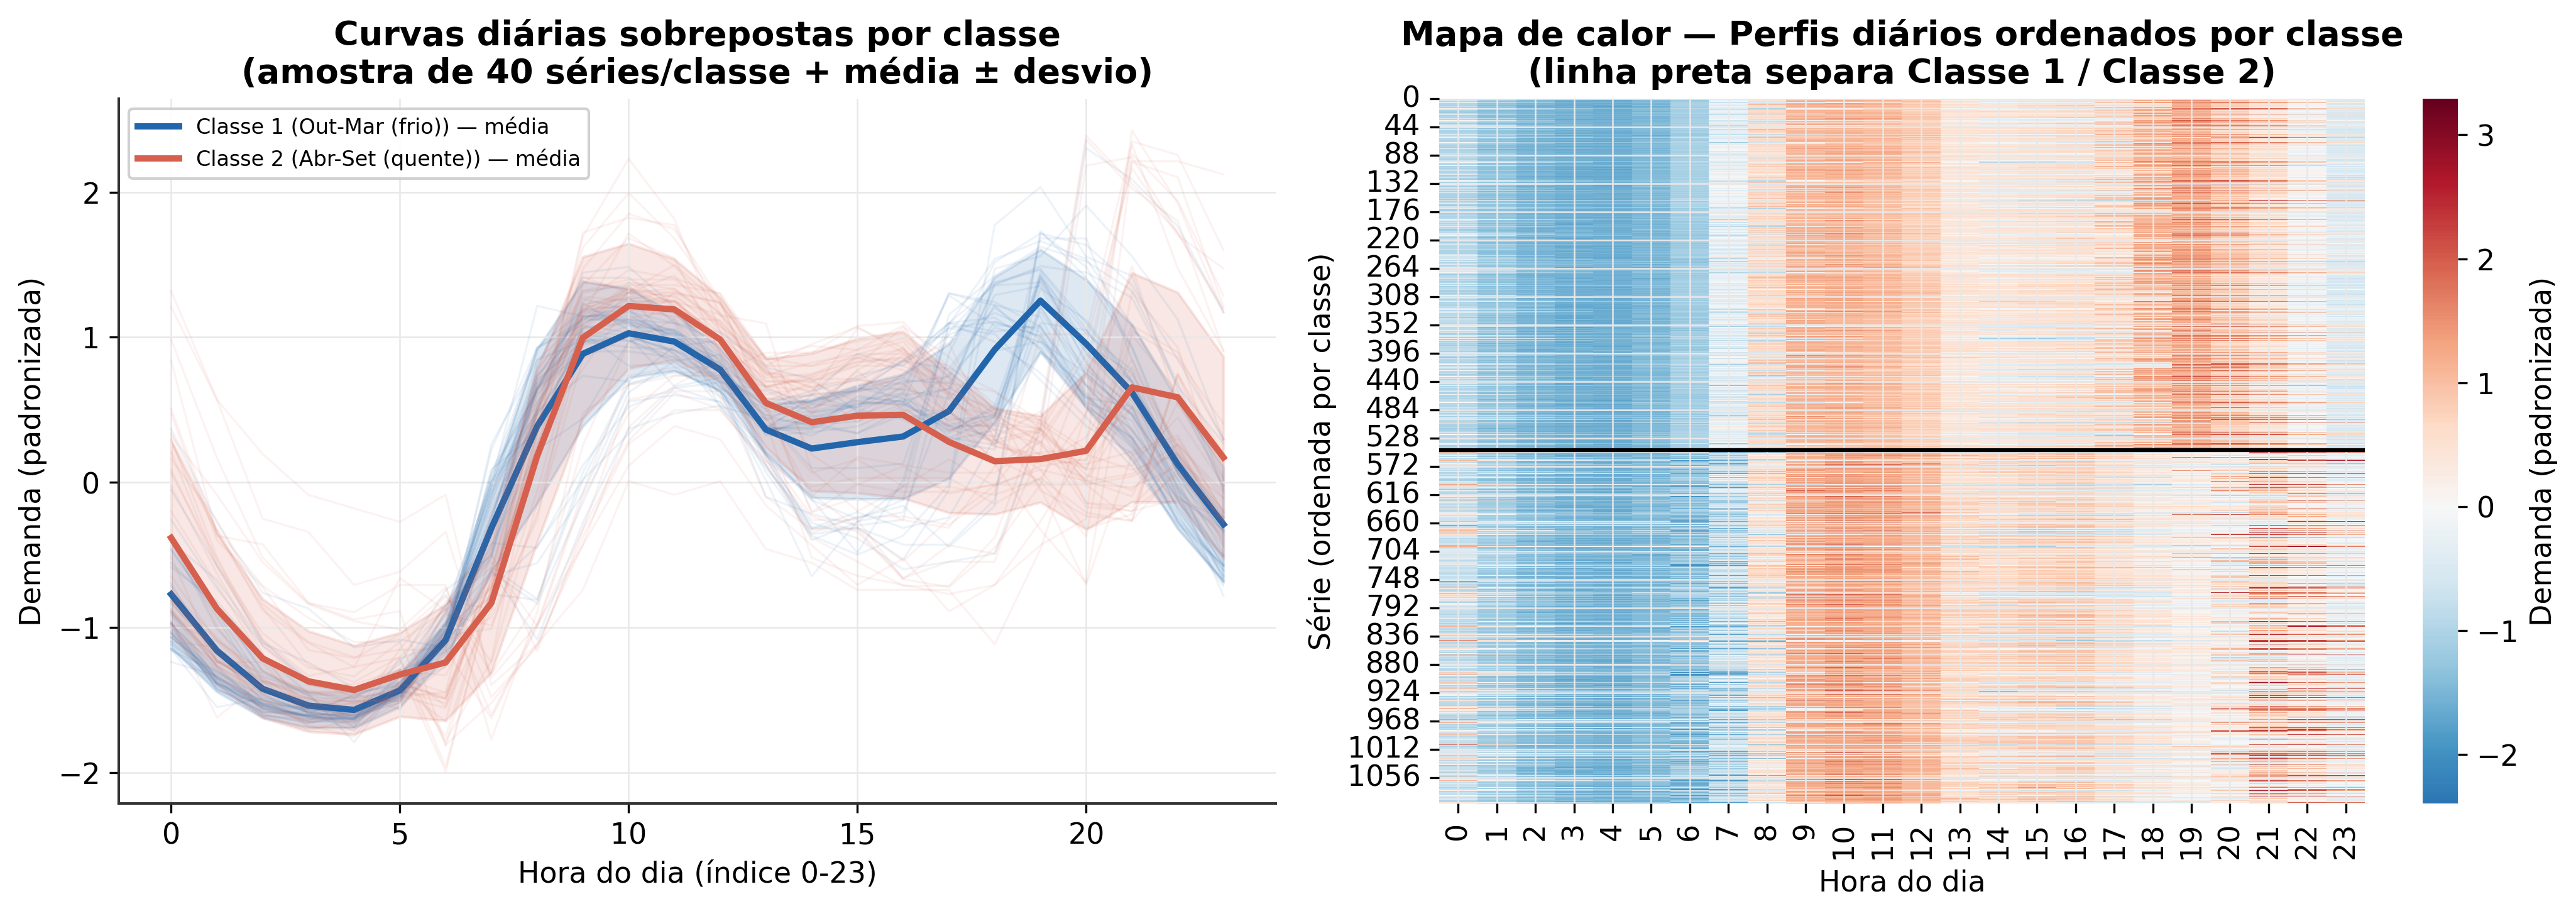
\includegraphics[width=0.85\textwidth]{Figuras_Aula2/fig8-series-heatmap.png}
    \caption{Curvas diárias sobrepostas e mapa de calor --- ItalyPowerDemand.}
    \label{fig:fig1}
\end{figure}


\subsection{Atributos extraídos}

\begin{table}[H]
\centering
\caption{Atributos extraídos por série --- média e desvio-padrão por classe}
\small
\begin{tabular}{lcccc}
\toprule
Atributo & Classe 1 (média) & Classe 1 (std) & Classe 2 (média) & Classe 2 (std) \\
\midrule
media           & $-0{,}000$ & 0{,}000 & 0{,}000  & 0{,}000 \\
desvio\_padrao  & 0{,}979 & 0{,}000 & 0{,}979 & 0{,}000 \\
pico            & 1{,}402 & 0{,}271 & 1{,}586 & 0{,}401 \\
hora\_do\_pico  & 16{,}00 & 4{,}18  & 12{,}48 & 4{,}63 \\
assimetria      & $-0{,}293$ & 0{,}349 & $-0{,}128$ & 0{,}444 \\
curtose         & $-1{,}164$ & 0{,}211 & $-0{,}938$ & 0{,}591 \\
fator\_de\_carga & $-0{,}000$ & 0{,}000 & 0{,}000 & 0{,}000 \\
\bottomrule
\end{tabular}
\end{table}

\subsection{Teste $t$, tamanho de efeito e informação mútua}

\begin{table}[H]
\centering
\caption{Ranking de atributos --- teste $t$ / Cohen's $d$ vs. Informação Mútua}
\begin{tabular}{lccc}
\toprule
Atributo & Cohen's $d$ & $|$Cohen's $d|$ & Informação Mútua \\
\midrule
hora\_do\_pico   & 0{,}7986  & 0{,}7986 & 0{,}3083 \\
pico             & $-0{,}5377$ & 0{,}5377 & 0{,}0754 \\
curtose          & $-0{,}5109$ & 0{,}5109 & 0{,}0732 \\
assimetria       & $-0{,}4129$ & 0{,}4129 & 0{,}1120 \\
media            & $-0{,}0898$ & 0{,}0898 & 0{,}0030 \\
fator\_de\_carga & $-0{,}0829$ & 0{,}0829 & 0{,}0260 \\
desvio\_padrao   & 0{,}0576  & 0{,}0576 & 0{,}0000 \\
\bottomrule
\end{tabular}
\end{table}

\noindent Correlação de Spearman entre os dois rankings ($|$Cohen's $d|$ vs. Informação Mútua): $\rho=0{,}857$ ($p=0{,}0137$), concordância razoável, com \texttt{hora\_do\_pico} no topo de ambos.


\begin{figure}[H]
    \centering
    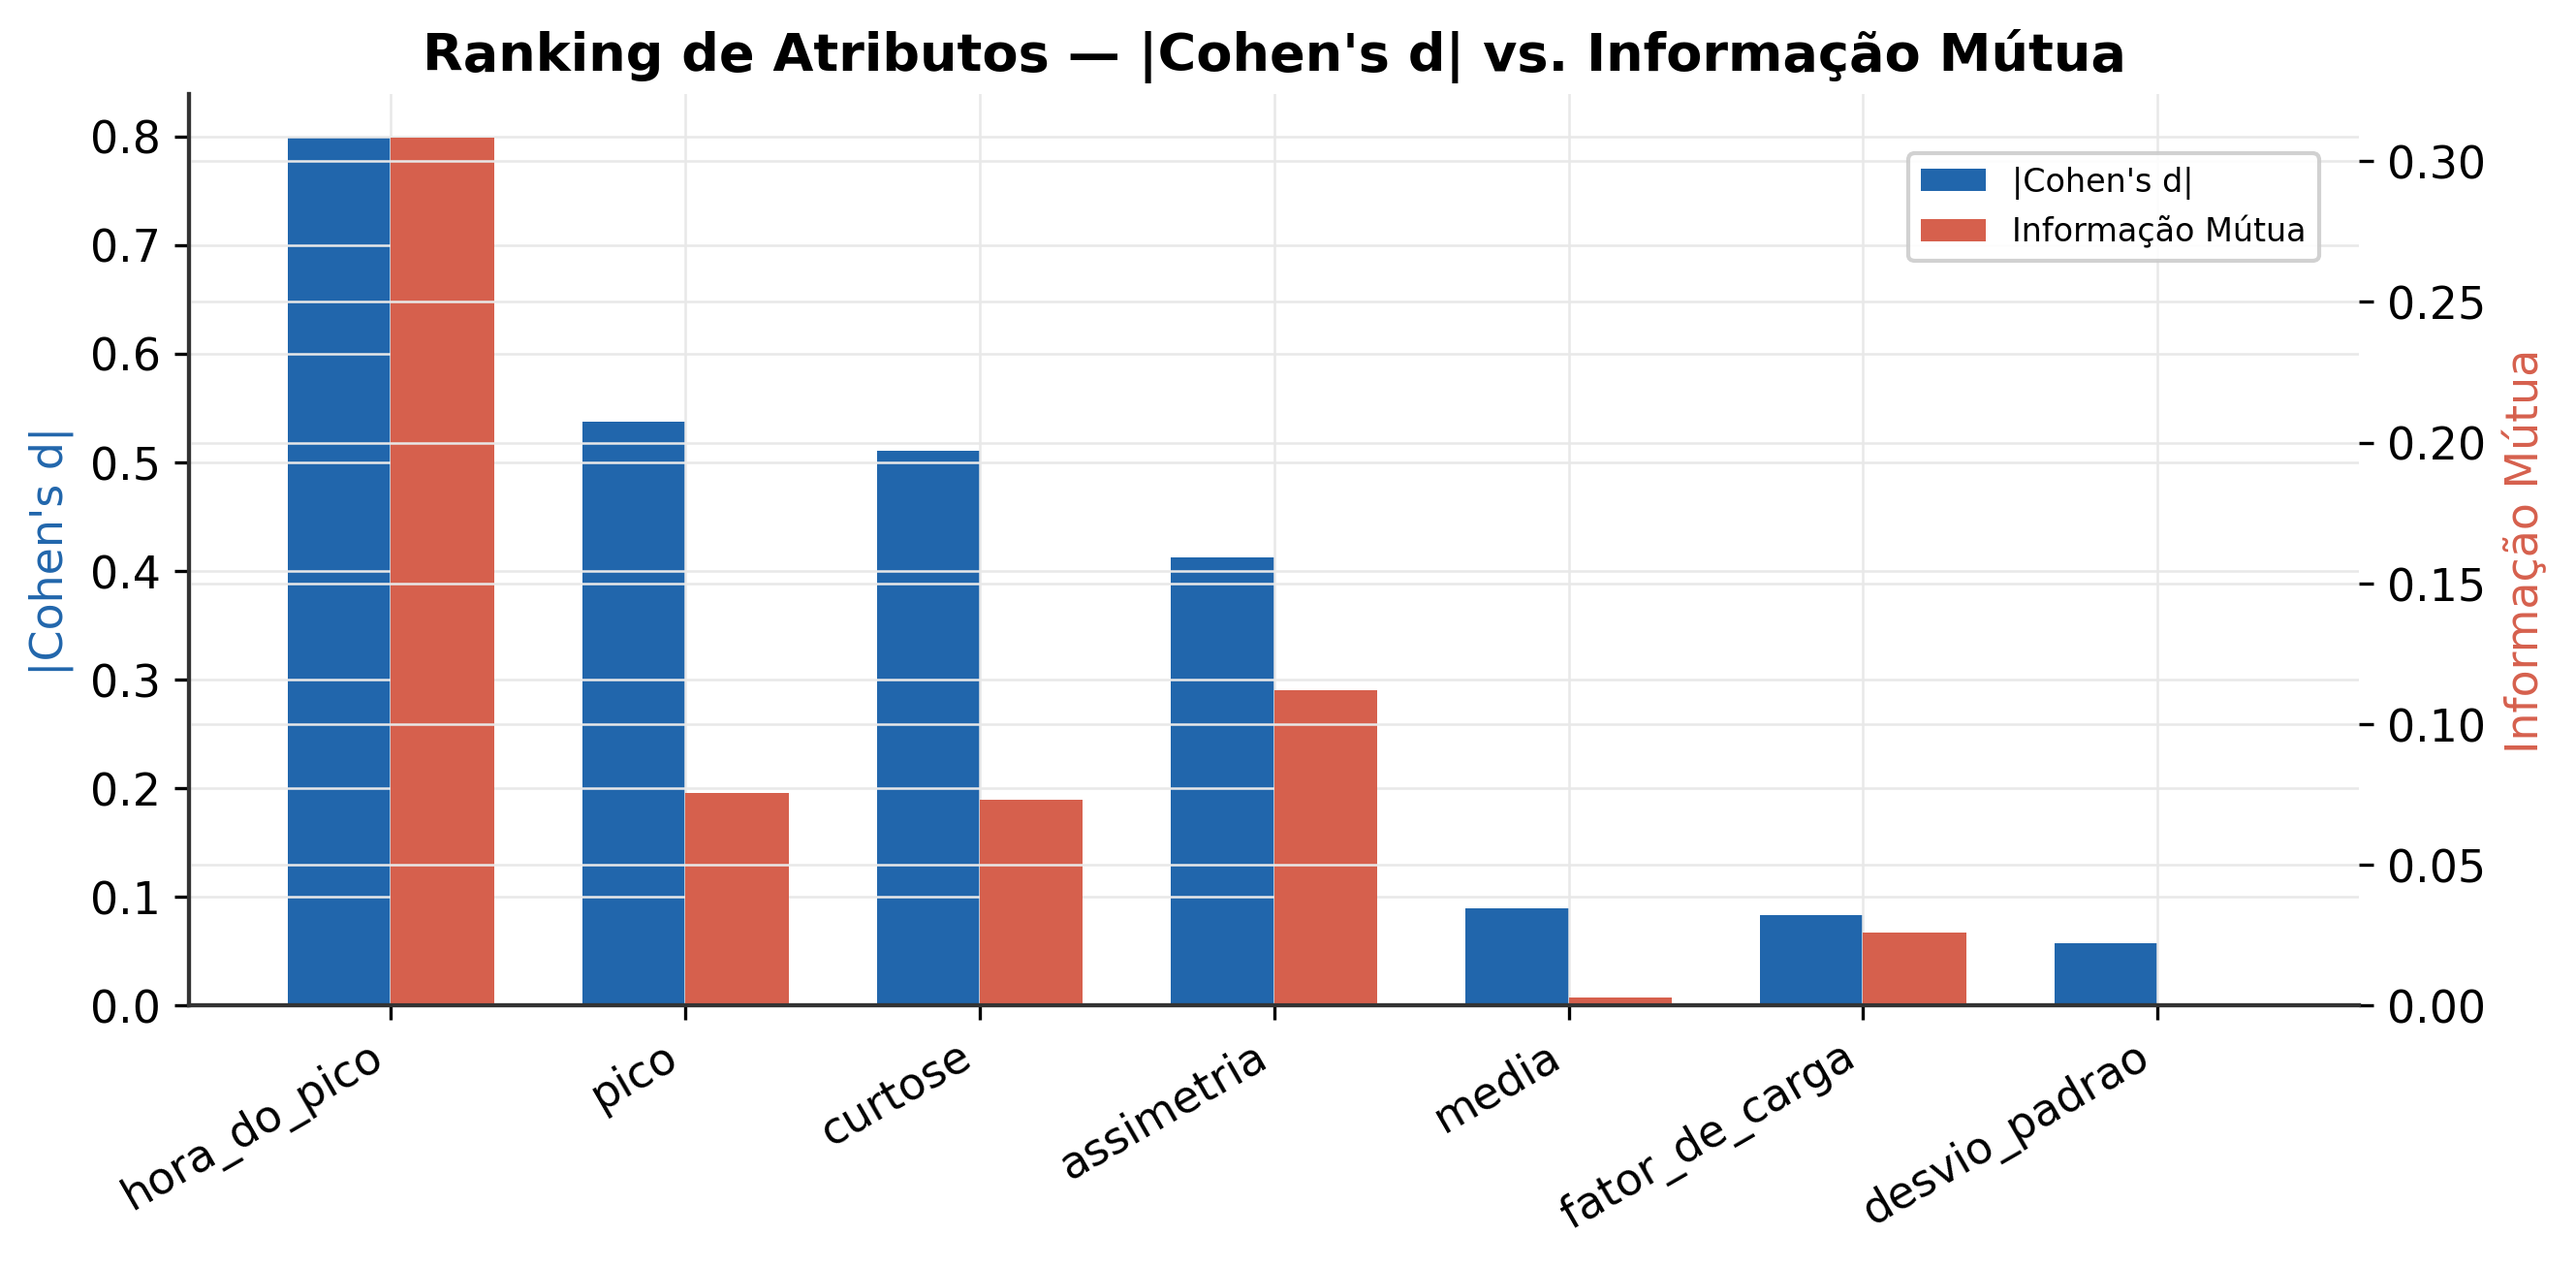
\includegraphics[width=0.85\textwidth]{Figuras_Aula2/fig9-ranking-atributos.png}
    \caption{Ranking de atributos --- $|$Cohen's $d|$ vs. Informação Mútua.}
    \label{fig:fig1}
\end{figure}



\subsection{Outliers multivariados --- distância de Mahalanobis}

\noindent \textbf{Nota metodológica:} a checagem de colinearidade revelou que \texttt{fator\_de\_carga} é quase perfeitamente correlacionado com \texttt{media} ($r\approx 0{,}99$) e \texttt{assimetria} correlaciona fortemente com \texttt{pico}/\texttt{curtose} ($r>0{,}8$). Essa colinearidade tornava a matriz de covariância quase singular, inflando artificialmente a distância de Mahalanobis (com os 7 atributos originais, $\sim$40\% dos pontos eram sinalizados como outliers, resultado não confiável). Por isso, usou-se um subconjunto de 5 atributos menos colineares (\texttt{media}, \texttt{desvio\_padrao}, \texttt{pico}, \texttt{hora\_do\_pico}, \texttt{curtose}) e \texttt{support\_fraction=0,9} no \texttt{MinCovDet}, para lidar com a assimetria de \texttt{pico}/\texttt{curtose}.

\begin{table}[H]
\centering
\caption{Outliers multivariados --- Mahalanobis por classe (limiar $\chi^2$, df=5, 97,5\%: 12,833)}
\begin{tabular}{lccc}
\toprule
Classe & Outliers & Total & \% \\
\midrule
1 (Out--Mar) & 40 & 547 & 7{,}3\% \\
2 (Abr--Set) & 85 & 549 & 15{,}5\% \\
\bottomrule
\end{tabular}
\end{table}

\subsection{PCA --- separabilidade das classes}

\noindent Variância explicada: PC1 = 44{,}7\%, PC2 = 29{,}5\%, total (2D) = 74{,}2\%.


\begin{figure}[H]
    \centering
    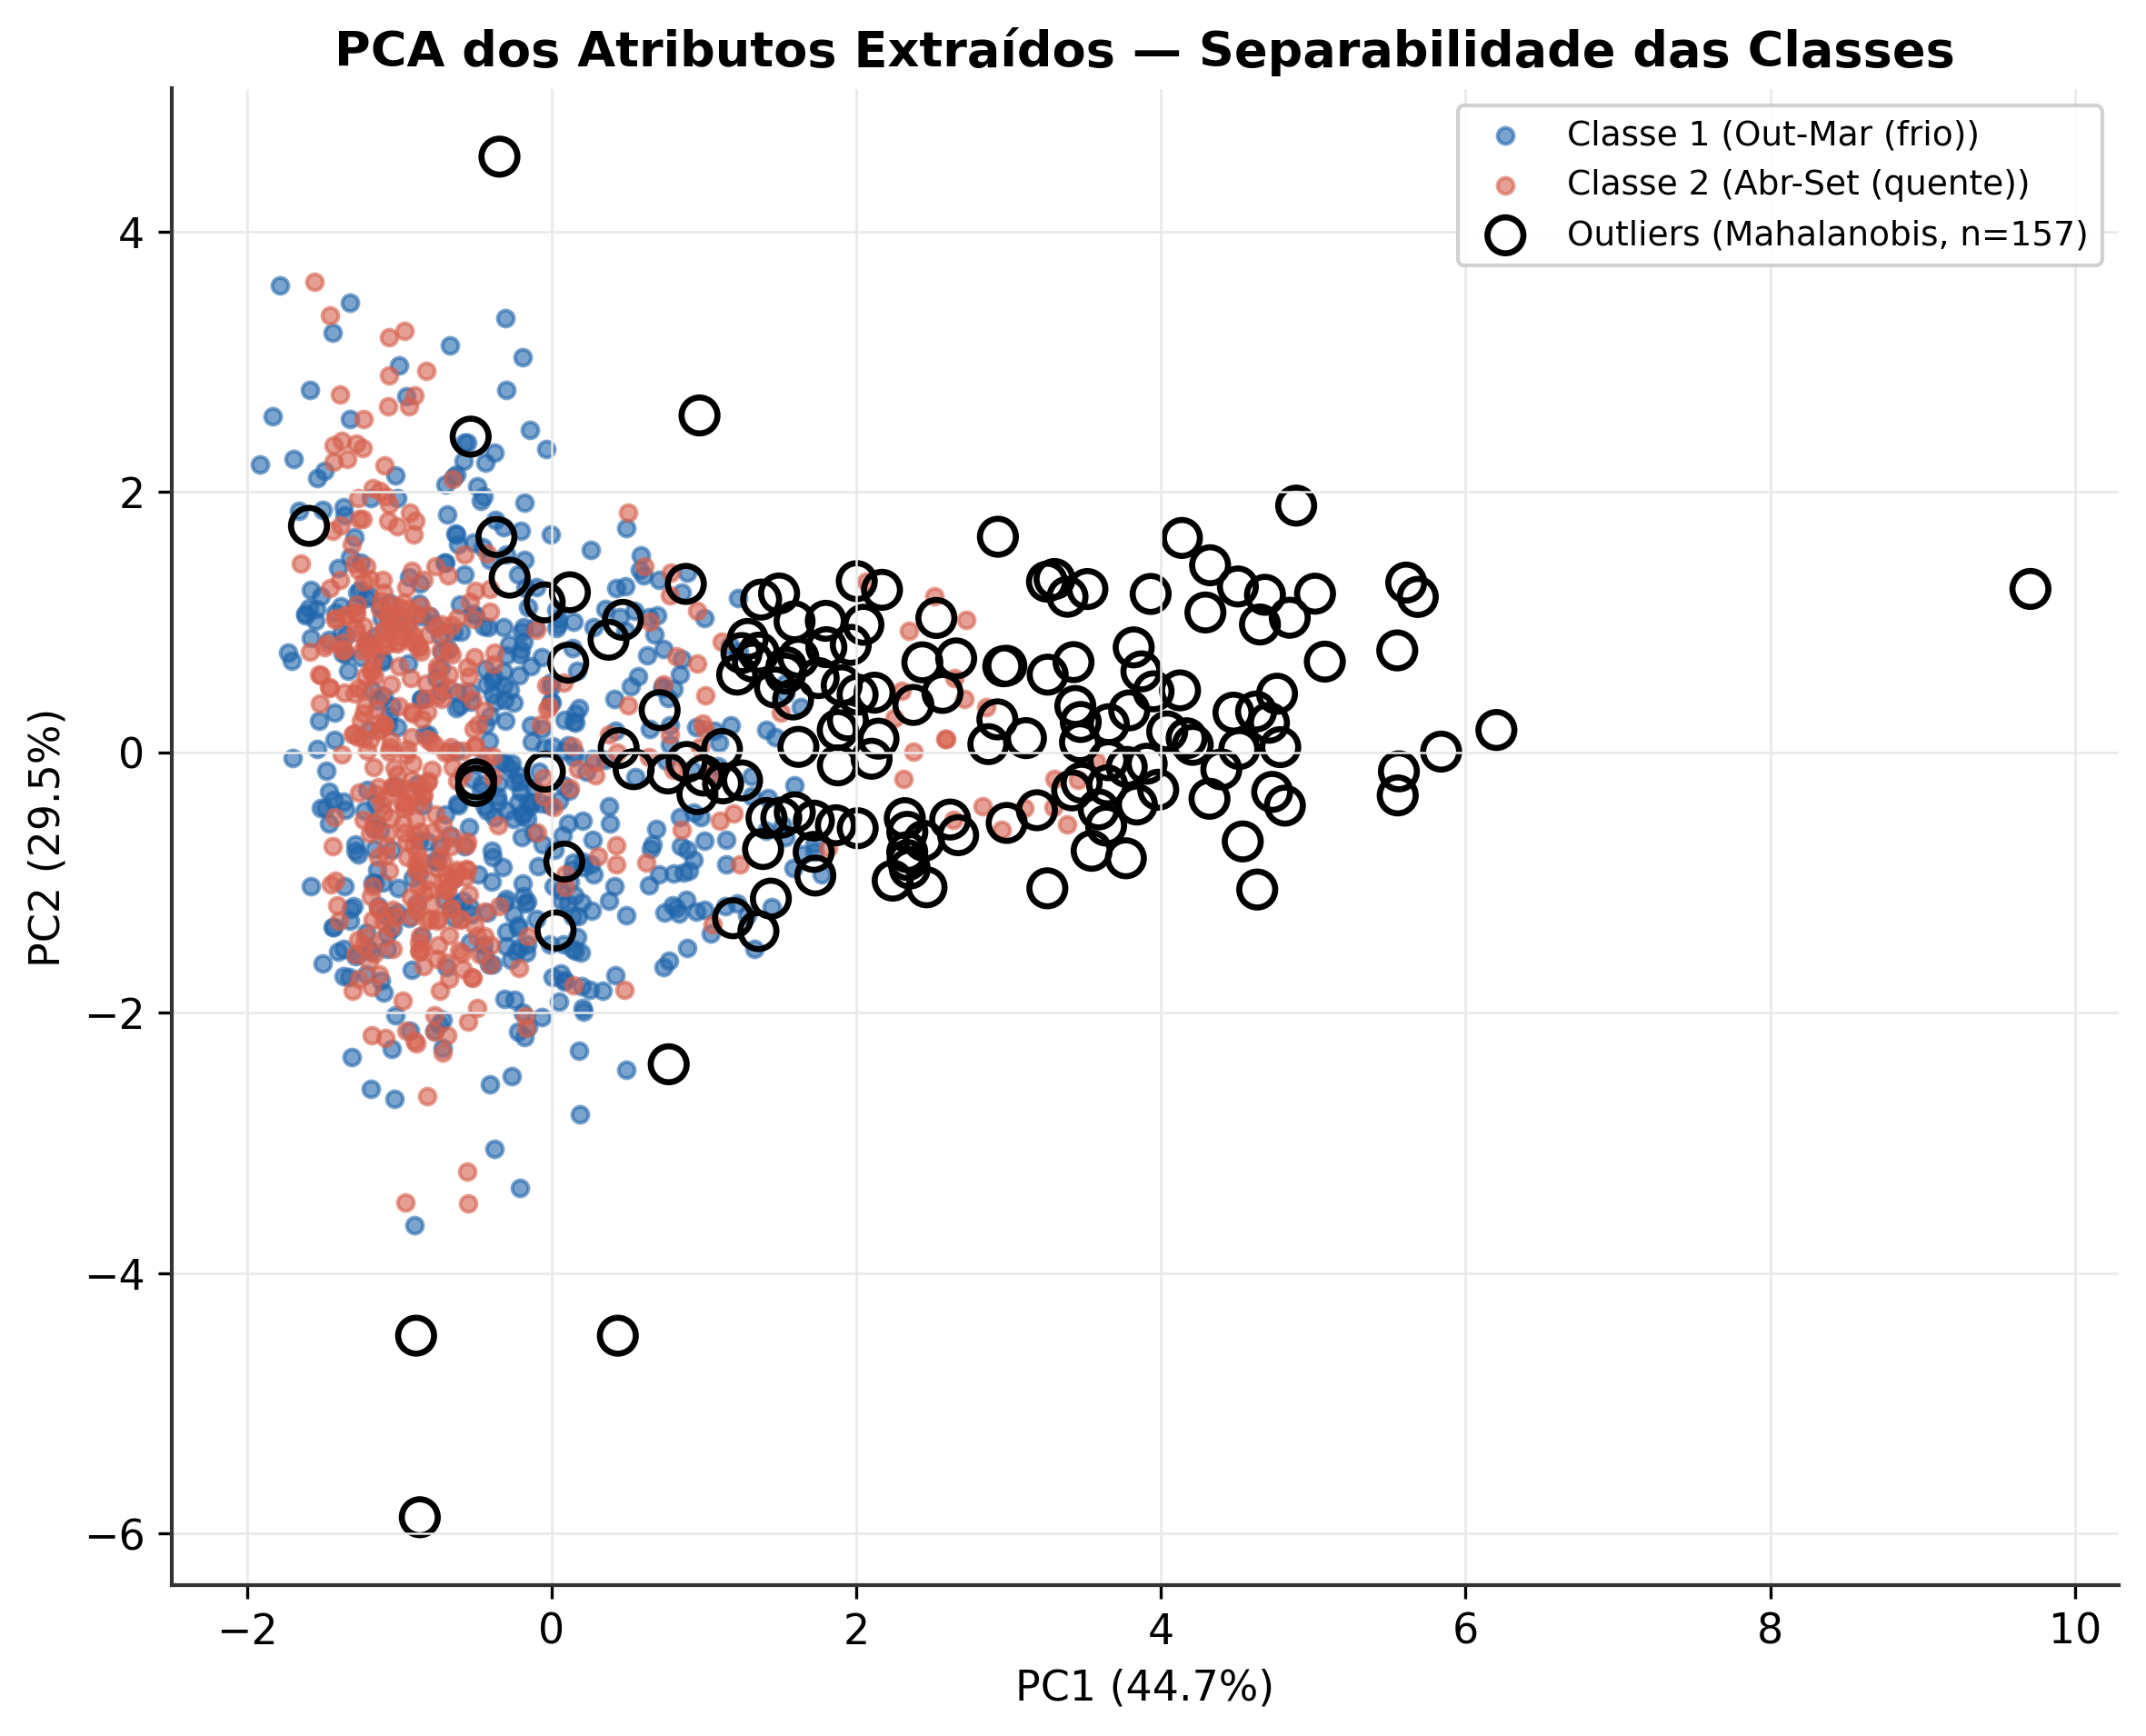
\includegraphics[width=0.85\textwidth]{Figuras_Aula2/fig10-pca-scatter.png}
    \caption{PCA dos atributos extraídos --- separabilidade das classes.}
    \label{fig:fig1}
\end{figure}

\subsection{Classificação --- comparação com baseline}

\begin{table}[H]
\centering
\caption{Comparação de classificadores vs. baseline}
\begin{tabular}{lcc}
\toprule
Modelo & Accuracy & F1-score \\
\midrule
Baseline (classe majoritária) & 0{,}5015 & 0{,}6680 \\
Logistic Regression           & 0{,}7903 & 0{,}8110 \\
K-NN (k=5)                    & 0{,}8237 & 0{,}8362 \\
Random Forest\textsuperscript{*} & 0{,}8511 & 0{,}8588 \\
\bottomrule
\end{tabular}
\\[0.2cm]
\footnotesize{\textsuperscript{*}Melhor classificador; ganho de 0{,}3495 sobre o baseline.}
\end{table}

\begin{figure}[H]
    \centering
    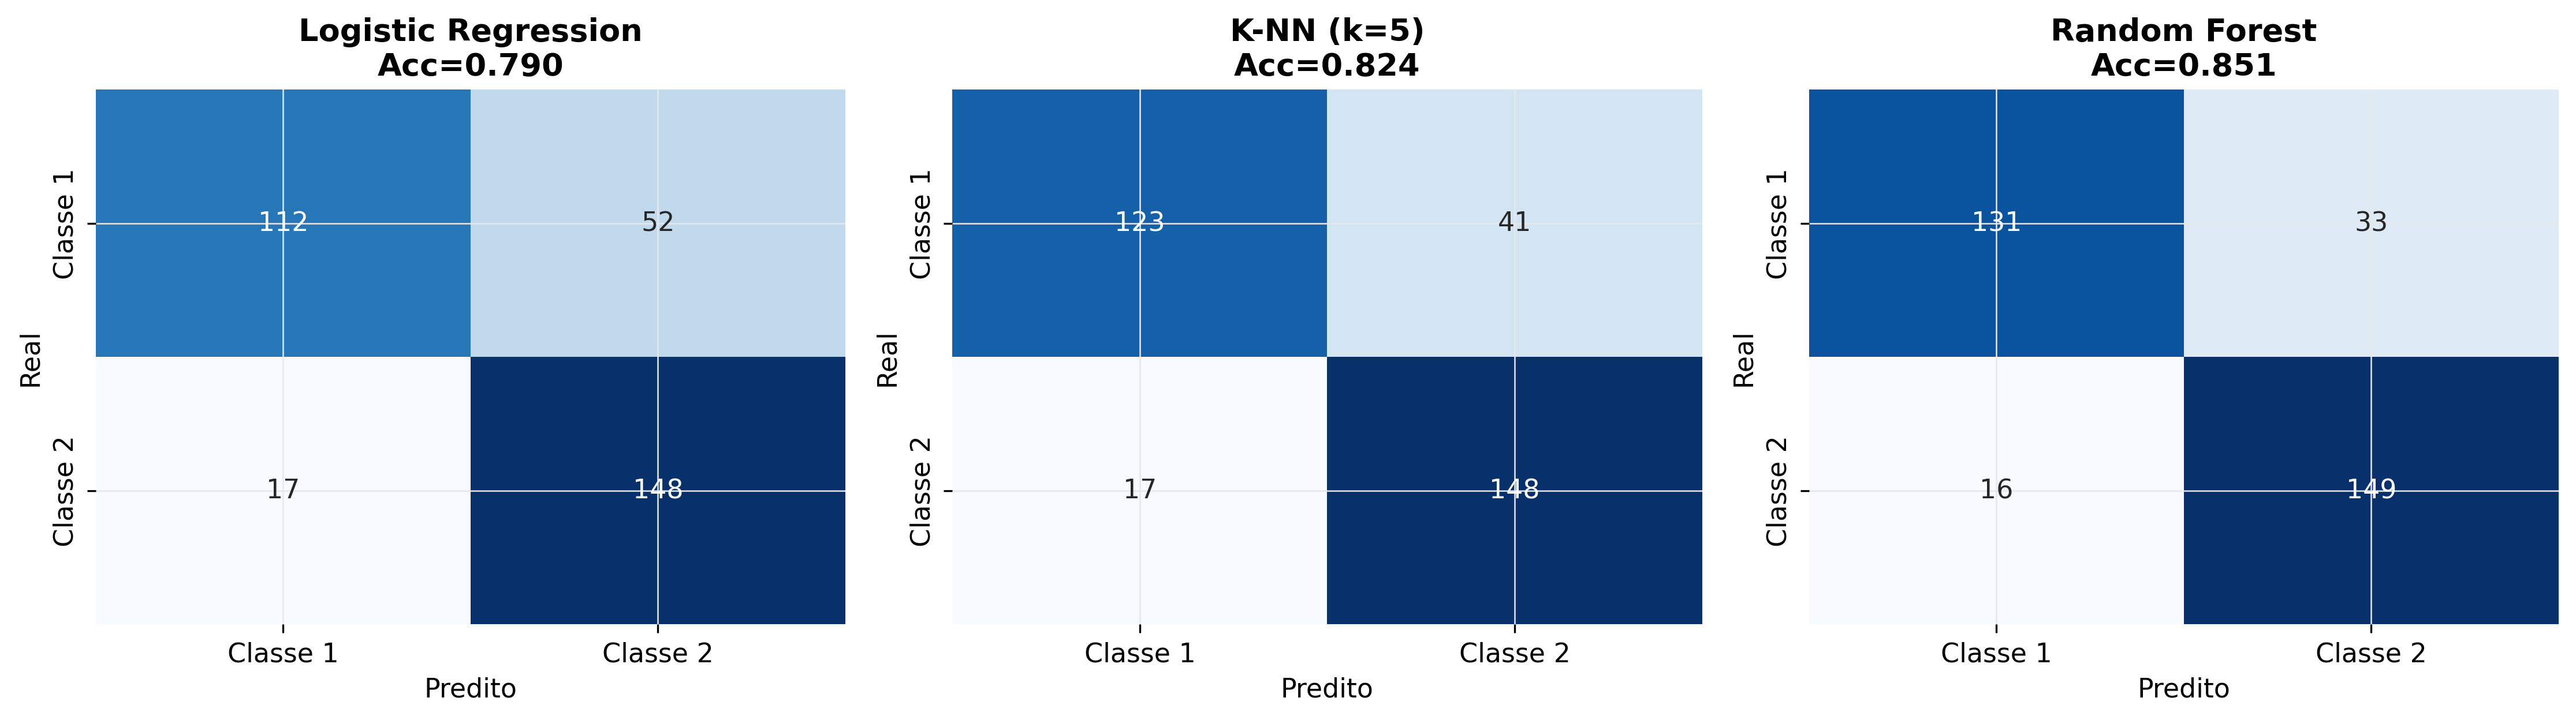
\includegraphics[width=0.85\textwidth]{Figuras_Aula2/fig11-matrizes-confusao-classificadores.png}
    \caption{Matrizes de confusão dos classificadores --- ItalyPowerDemand.}
    \label{fig:fig1}
\end{figure}

\subsection{Discussão final}

Os atributos extraídos, especialmente \texttt{hora\_do\_pico} (maior $|$Cohen's $d|$ e maior Informação Mútua), foram suficientes para separar bem as classes: a projeção em PCA (74,2\% de variância em 2D) já mostra separação visual clara, e o Random Forest superou o baseline em quase 35 pontos percentuais de accuracy. Os outliers multivariados (mais frequentes na classe 2, Abr--Set) provavelmente correspondem a dias cuja curva de demanda foge do padrão típico da própria estação. Técnicas mais sofisticadas, atributos espectrais via FFT, \emph{Dynamic Time Warping} (DTW) ou redes 1D-CNN, poderiam melhorar ainda mais os resultados, mas o ganho marginal tende a ser pequeno neste dataset, um dos mais ``fáceis'' do UCR Archive.

\newpage
% ============================================================
% CONCLUSÃO GERAL
% ============================================================
\section{Considerações Finais}

Os dois exercícios desta lista demonstram, sobre dados reais, o roteiro completo de EDA para séries temporais: qualidade dos dados $\rightarrow$ univariada $\rightarrow$ outliers $\rightarrow$ tendência/sazonalidade $\rightarrow$ padrões cíclicos $\rightarrow$ autocorrelação $\rightarrow$ frequência $\rightarrow$ estacionariedade $\rightarrow$ relações bivariadas/multivariadas. No caso da carga elétrica PJM, a EDA revelou uma dupla sazonalidade (diária + semanal) que exige tratamento explícito (múltiplas sazonalidades ou termos de Fourier) para modelos de previsão. No caso do ItalyPowerDemand, a EDA orientada à classificação mostrou que um pequeno conjunto de atributos interpretáveis, extraídos com cuidado metodológico (evitando colinearidade), já é suficiente para uma classificação de alta qualidade.

\end{document}